\chapter*{Le Kerala de Cochin à Munnar\markboth{Le Kerala de Cochin à Munnar}{}}
\section*{8 novembre 2015}
J'atteris à Cochin, sur la côte ouest au sud de l'Inde 

 Visite de Fort Kochi, ancienne ville coloniale hollandaise, célèbre pour ses filets de pêche chinois 

 

\begin{center} 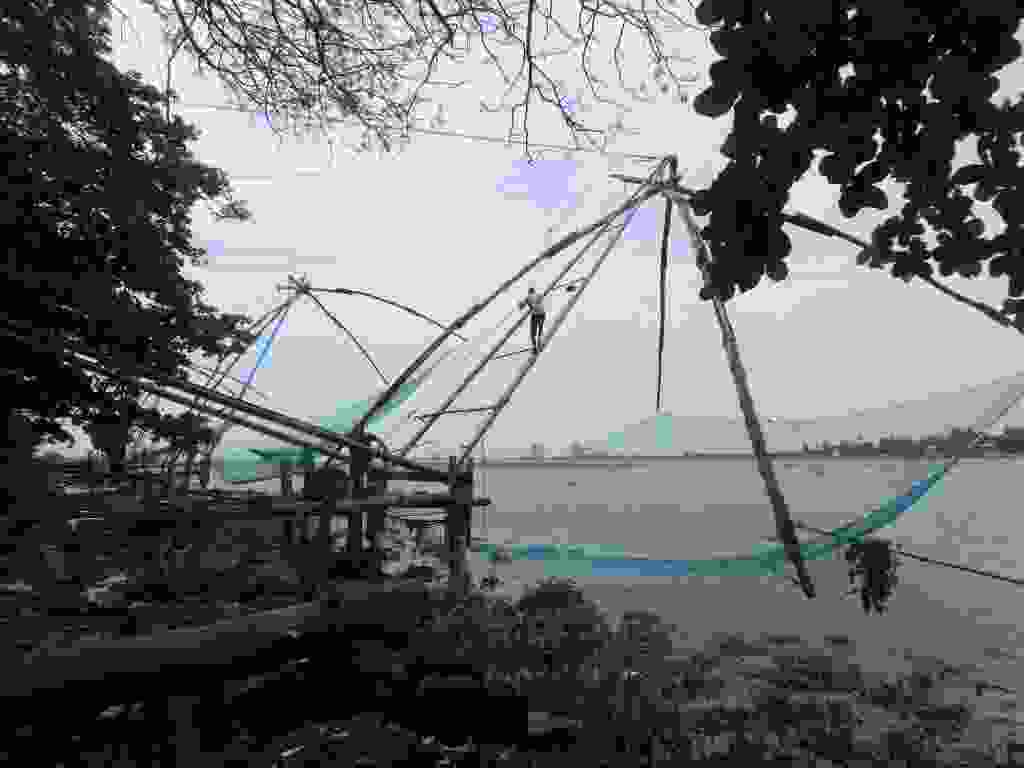
\includegraphics[width=\mywidth]{../wp-content/uploads/2015/11/wpid-oi000179-1024x768.jpg} \end{center}

 

 

\begin{center} 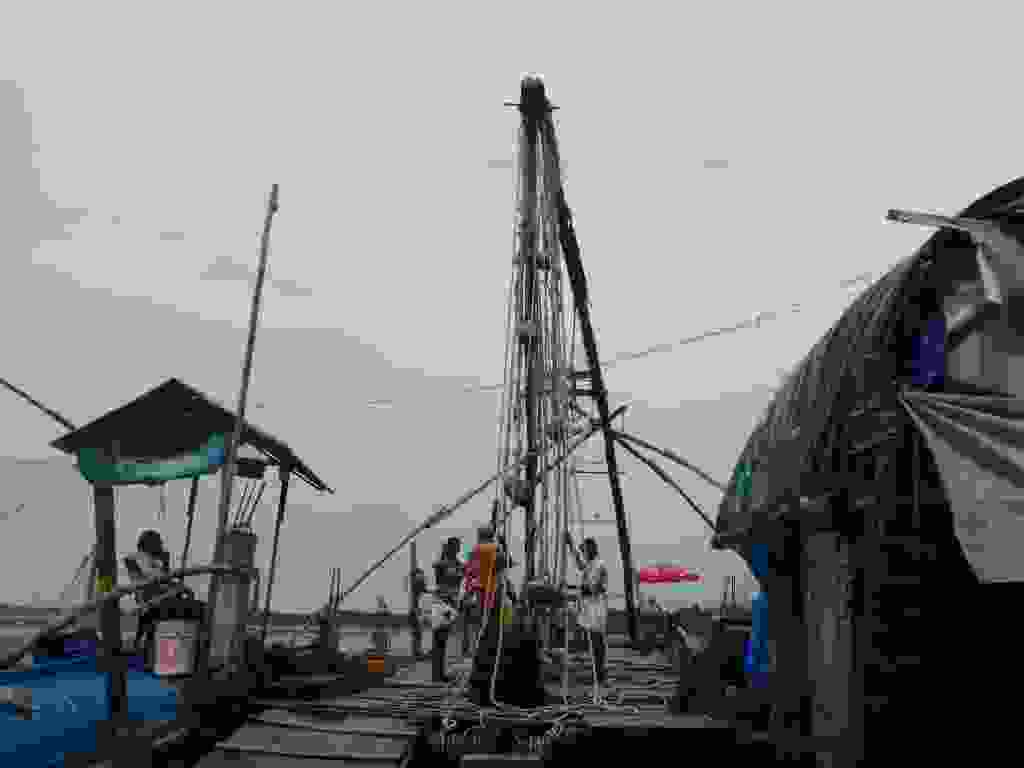
\includegraphics[width=\mywidth]{../wp-content/uploads/2015/11/wpid-oi000181-1024x768.jpg} \end{center}

 

 

\begin{center} 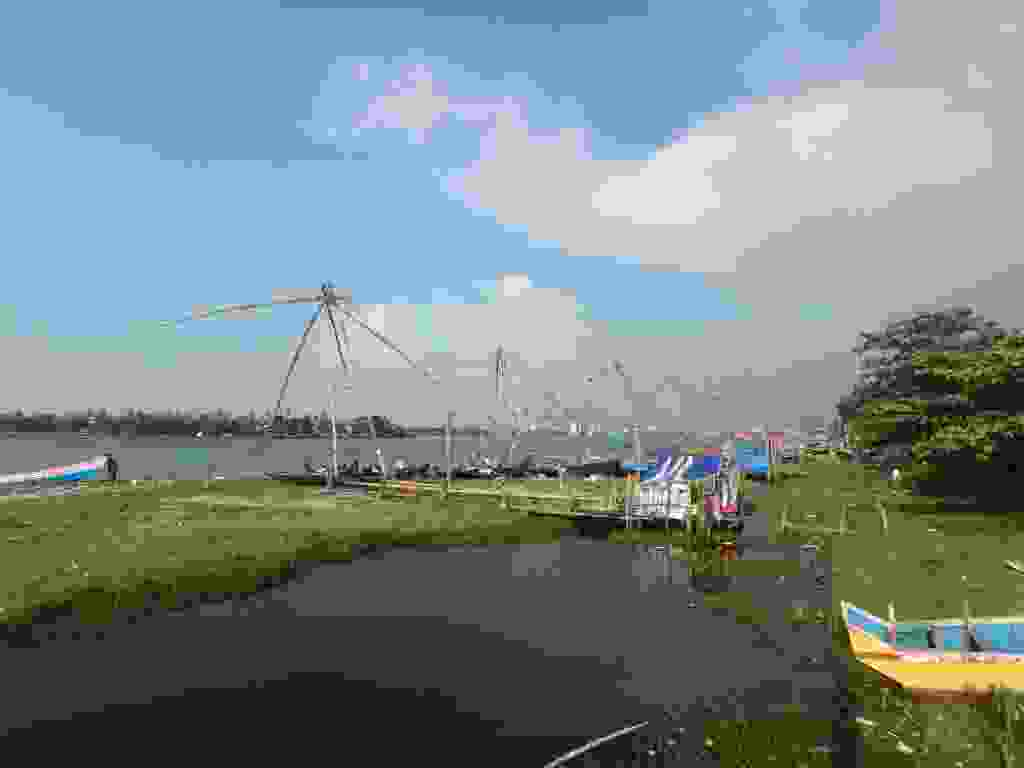
\includegraphics[width=\mywidth]{../wp-content/uploads/2015/11/wpid-oi000218-1024x768.jpg} \end{center}

 

 Le palais hollandais, de belles peintures murales à l'intérieur mais photos interdites 

 

\begin{center} 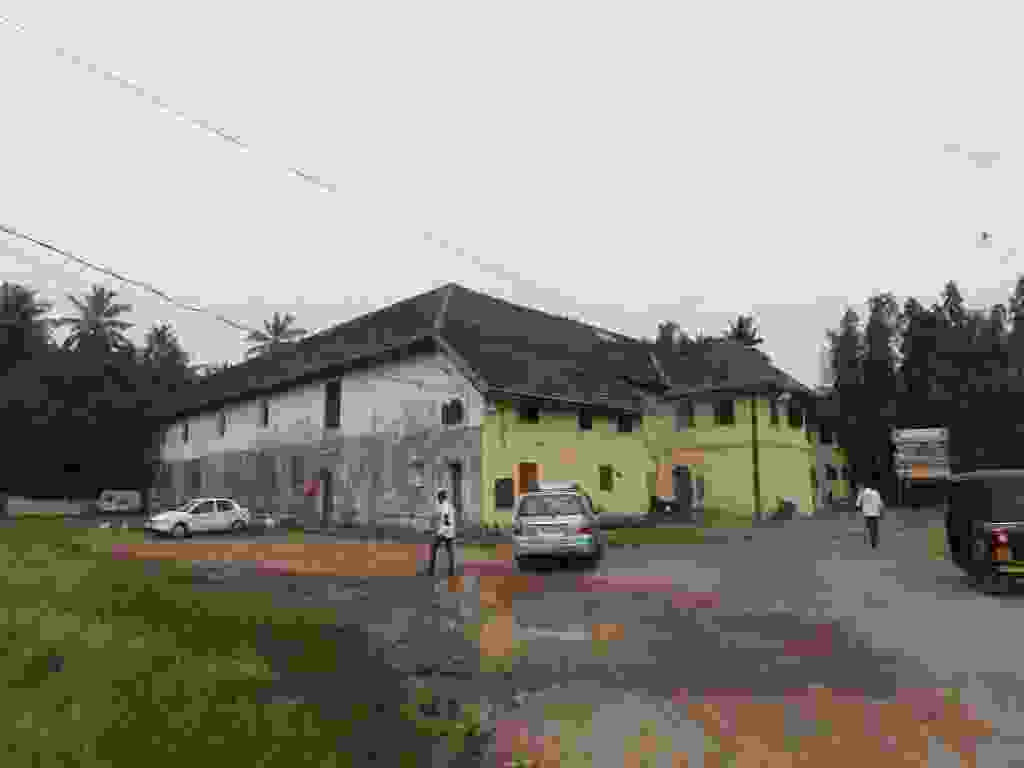
\includegraphics[width=\mywidth]{../wp-content/uploads/2015/11/wpid-oi000194-1024x768.jpg} \end{center}

 

 Église St Francis où Vasco de Gama a été enterré 

 

\begin{center} 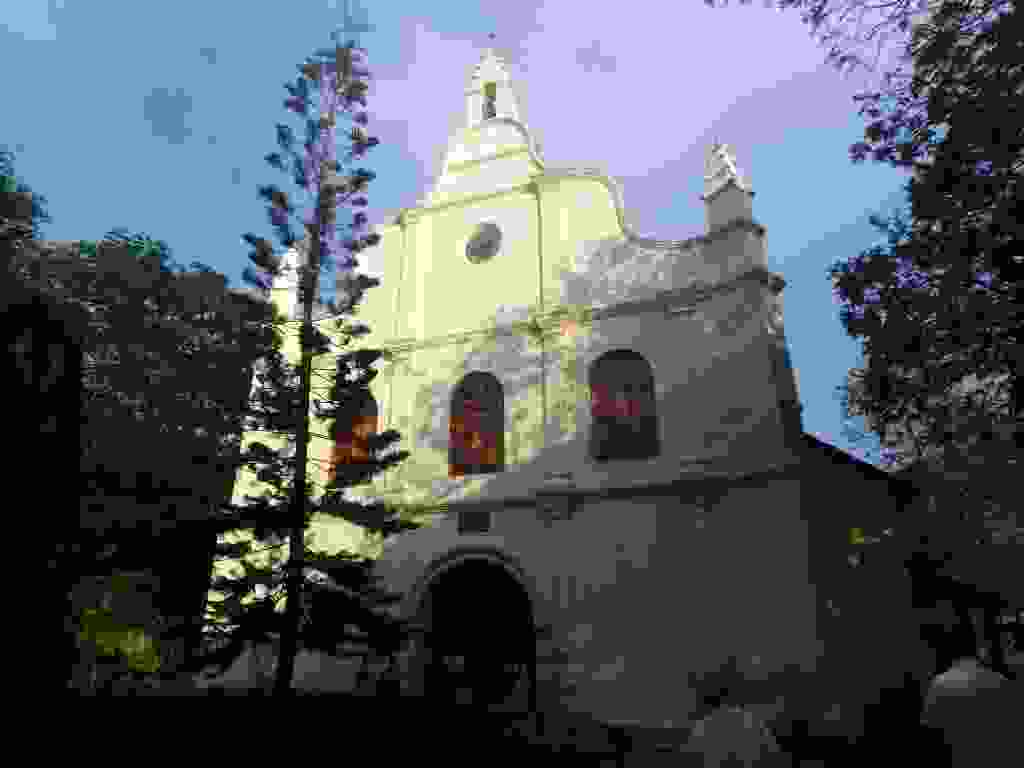
\includegraphics[width=\mywidth]{../wp-content/uploads/2015/11/wpid-oi000215-1024x768.jpg} \end{center}

 

 Quartier juif avec une très ancienne synagogue et des rues commerçantes 

 

\begin{center} 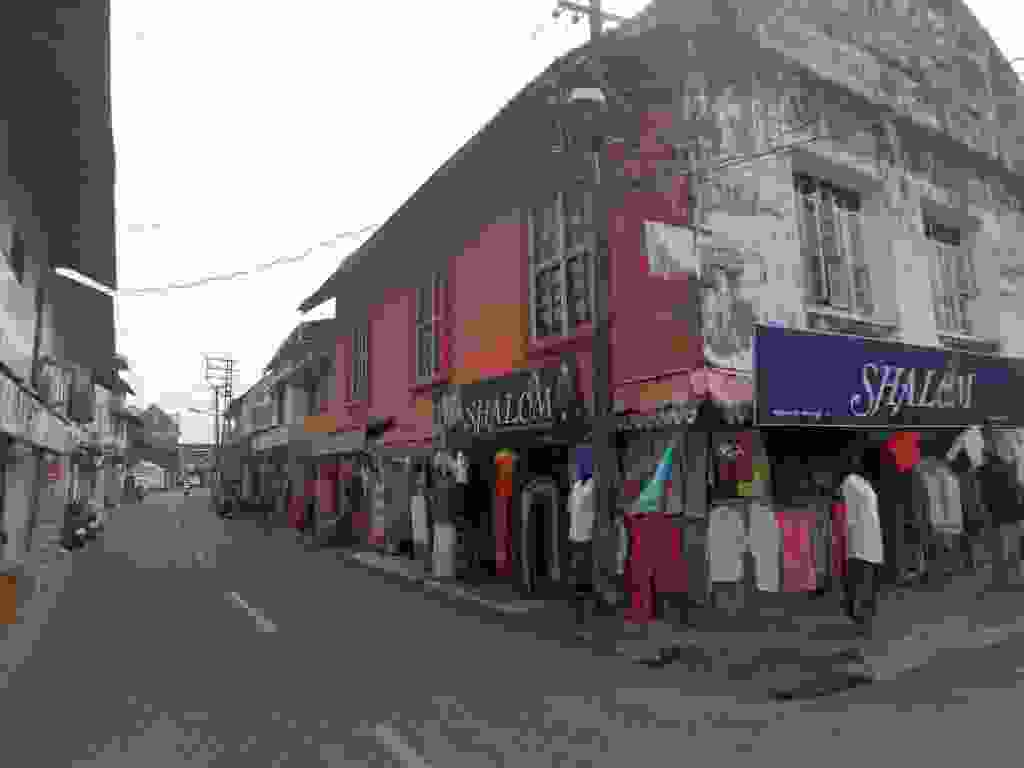
\includegraphics[width=\mywidth]{../wp-content/uploads/2015/11/wpid-oi000197-1024x768.jpg} \end{center}

 

 

\begin{center} 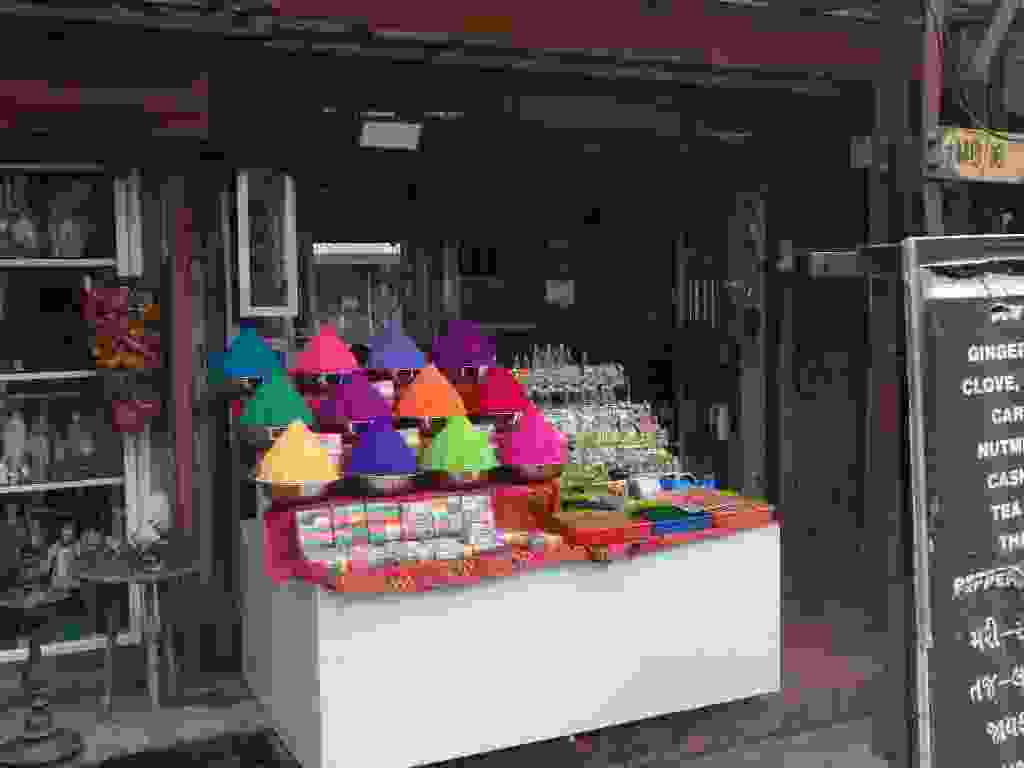
\includegraphics[width=\mywidth]{../wp-content/uploads/2015/11/wpid-oi000196-1024x768.jpg} \end{center}

 

 Les rickshaws qui proposent des tours gratuits à condition d'entrer dans une boutique de souvenirs 

 

\begin{center} 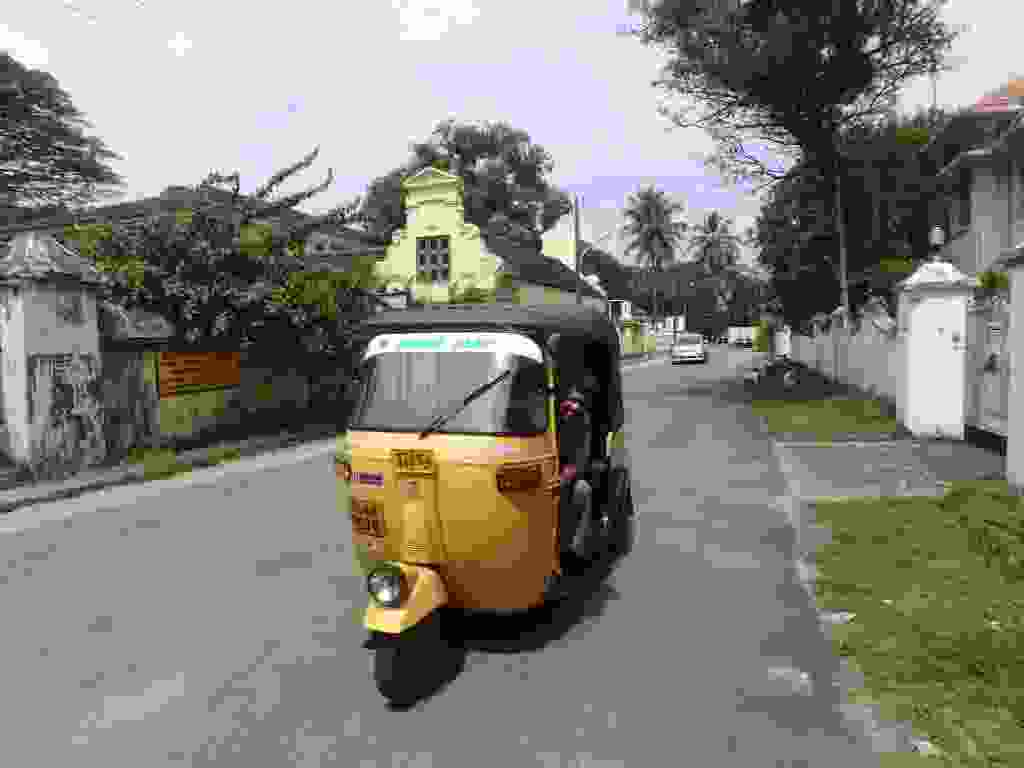
\includegraphics[width=\mywidth]{../wp-content/uploads/2015/11/wpid-oi000186-1024x768.jpg} \end{center}

 

 Je rejoins ensuite un groupe de «vacanciers» toulousains, l'occasion de faire du yoga dans un cadre agréable 

 

\begin{center} 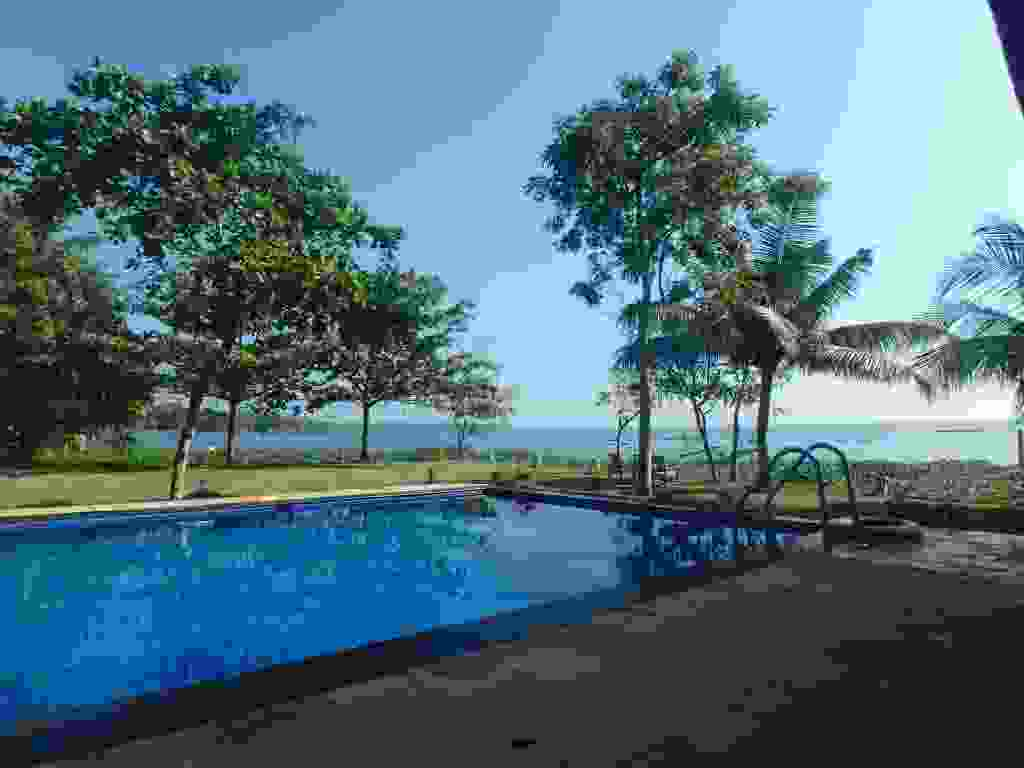
\includegraphics[width=\mywidth]{../wp-content/uploads/2015/11/wpid-oi000210-1024x768.jpg} \end{center}

 

 

\begin{center} 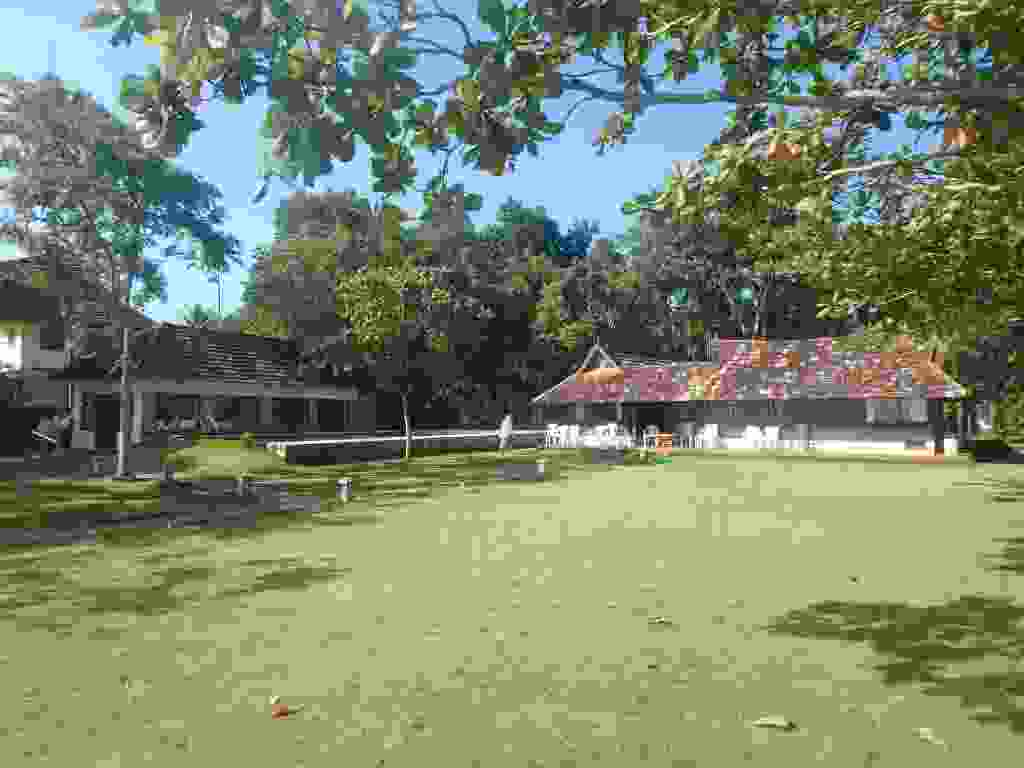
\includegraphics[width=\mywidth]{../wp-content/uploads/2015/11/wpid-oi000212-1024x768.jpg} \end{center}

 

 Et une excursion en bateau dans les backwaters 

 

\begin{center} 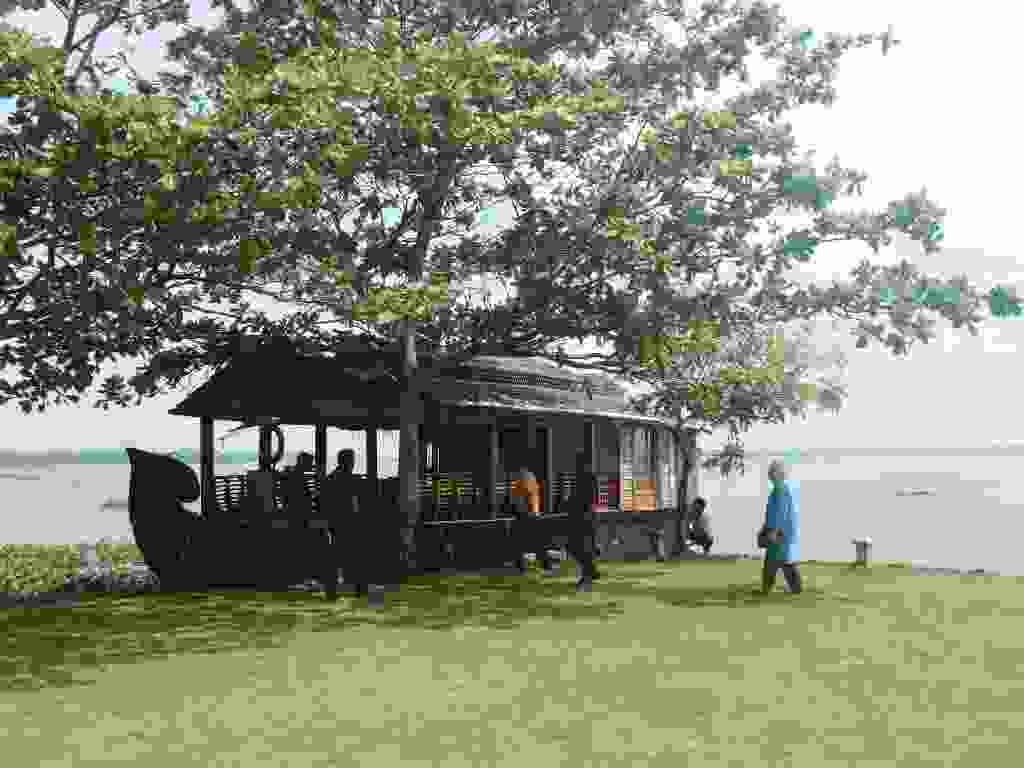
\includegraphics[width=\mywidth]{../wp-content/uploads/2015/11/wpid-oi000221-1024x768.jpg} \end{center}

 

 

\begin{center} 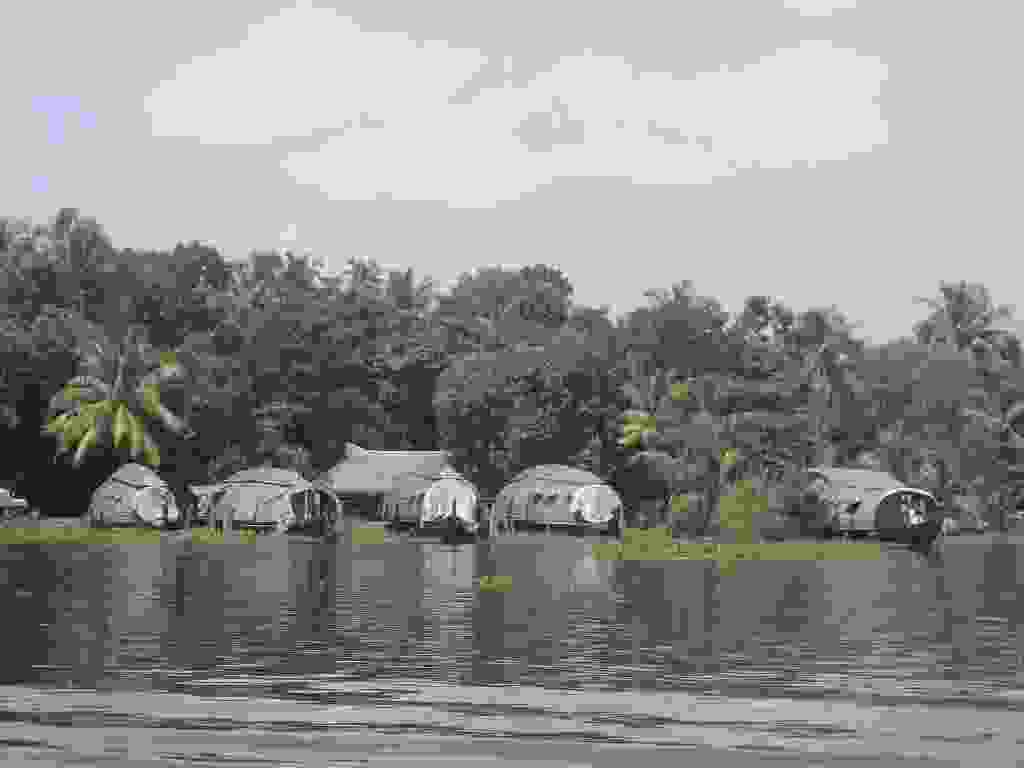
\includegraphics[width=\mywidth]{../wp-content/uploads/2015/11/wpid-oi000226-1024x768.jpg} \end{center}

 

 

\begin{center} 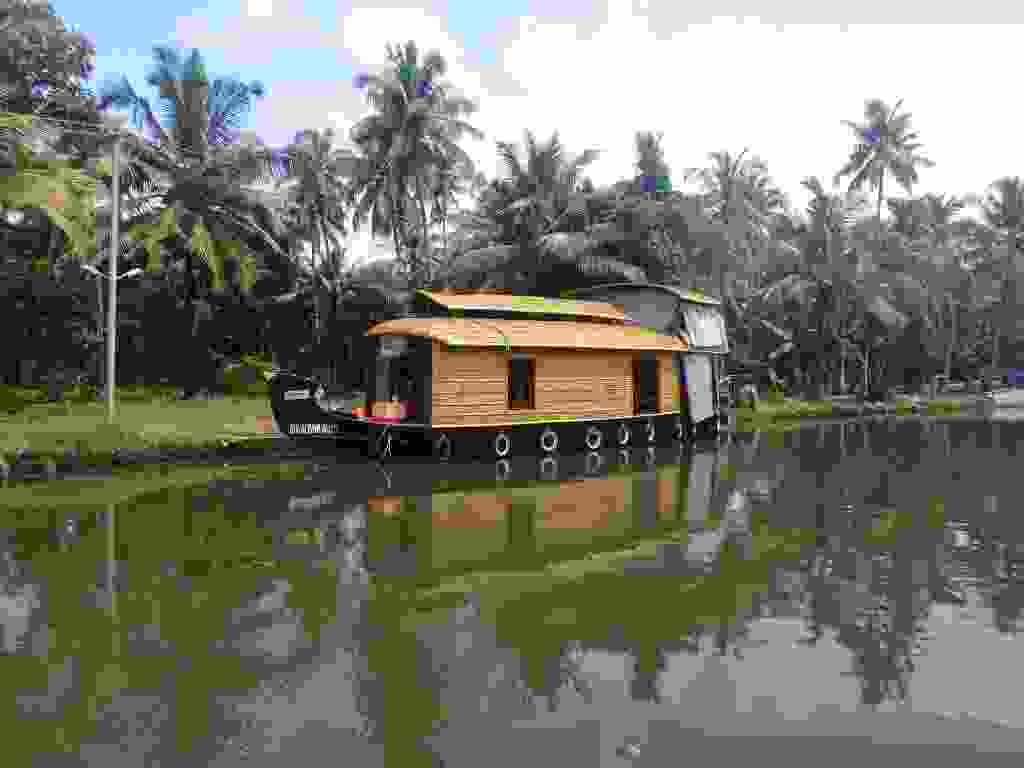
\includegraphics[width=\mywidth]{../wp-content/uploads/2015/11/wpid-oi000234-1024x768.jpg} \end{center}

 

 

\begin{center} 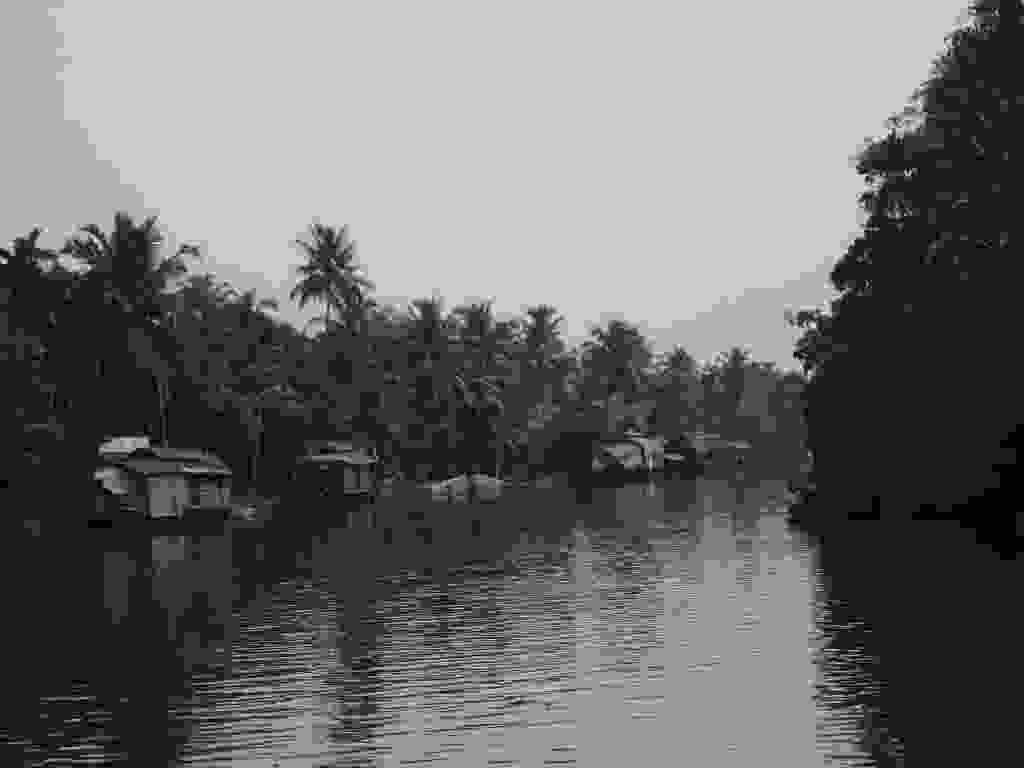
\includegraphics[width=\mywidth]{../wp-content/uploads/2015/11/wpid-oi000233-1024x768.jpg} \end{center}

 

 

\begin{center} 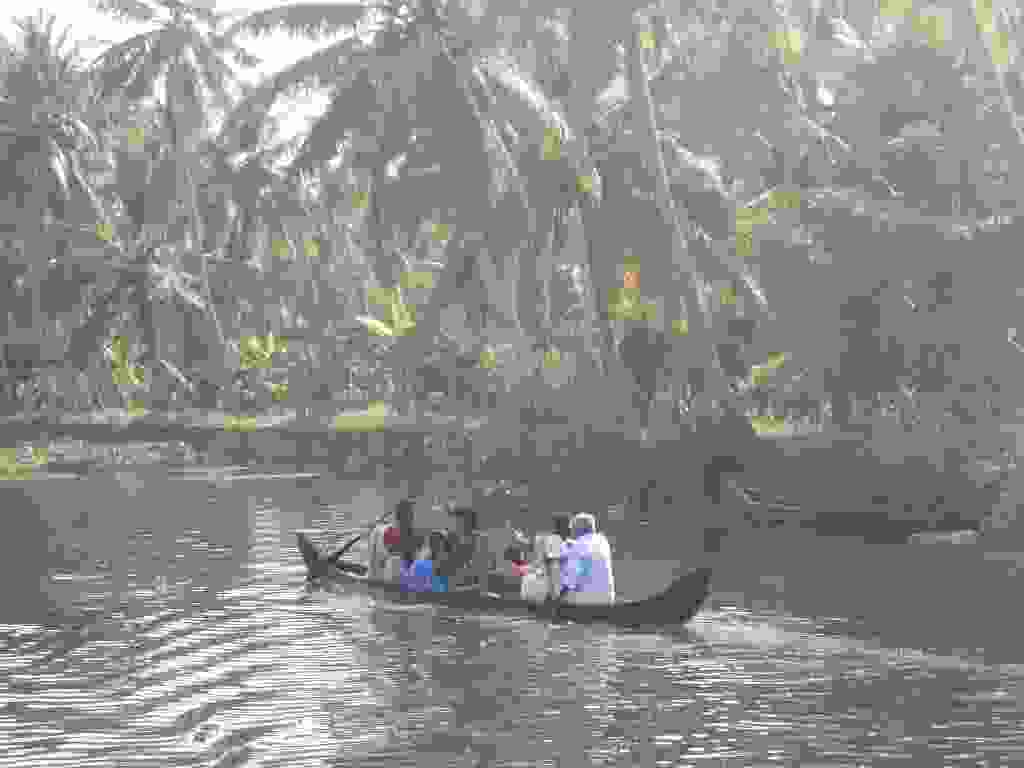
\includegraphics[width=\mywidth]{../wp-content/uploads/2015/11/wpid-oi000245-1024x768.jpg} \end{center}

 

 

\begin{center} 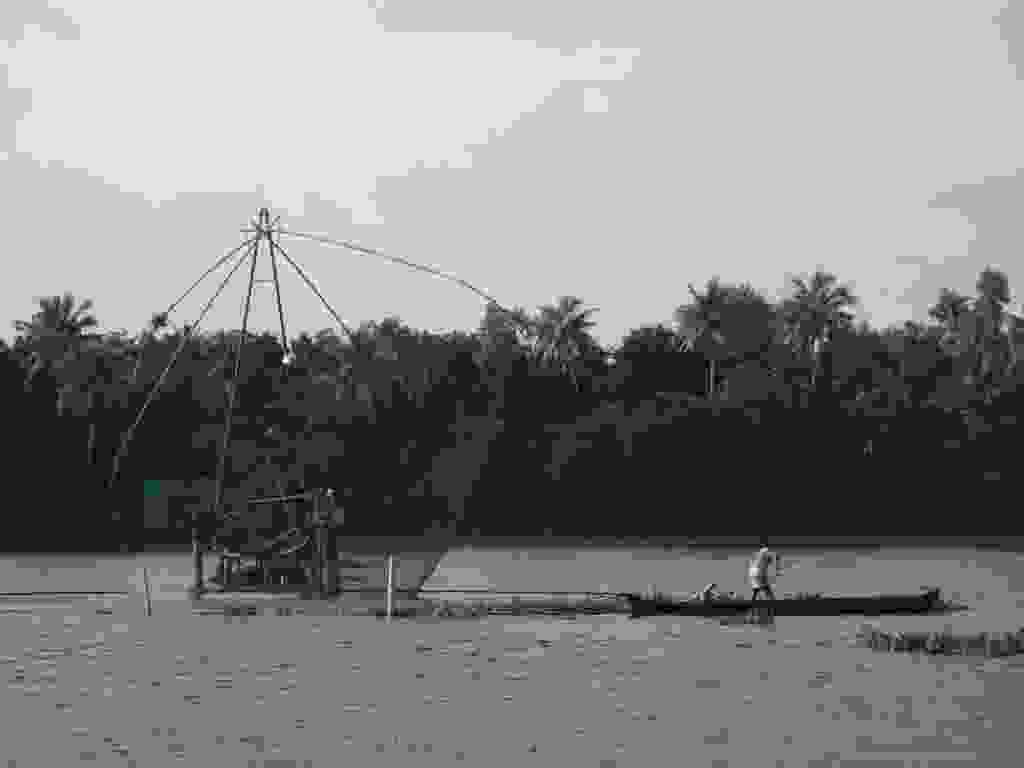
\includegraphics[width=\mywidth]{../wp-content/uploads/2015/11/wpid-oi000250-1024x768.jpg} \end{center}

 

 Des femmes font la lessive en frappant le linge sur une pierre 

 

\begin{center} 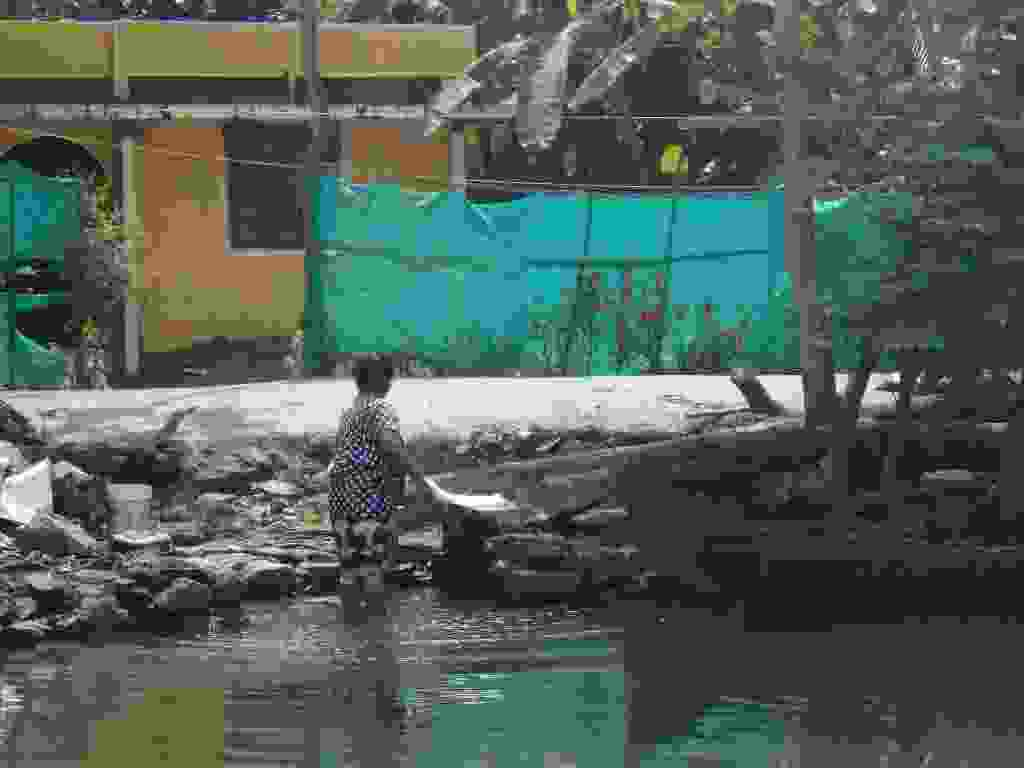
\includegraphics[width=\mywidth]{../wp-content/uploads/2015/11/wpid-oi000239-1024x768.jpg} \end{center}

 

 

\begin{center} 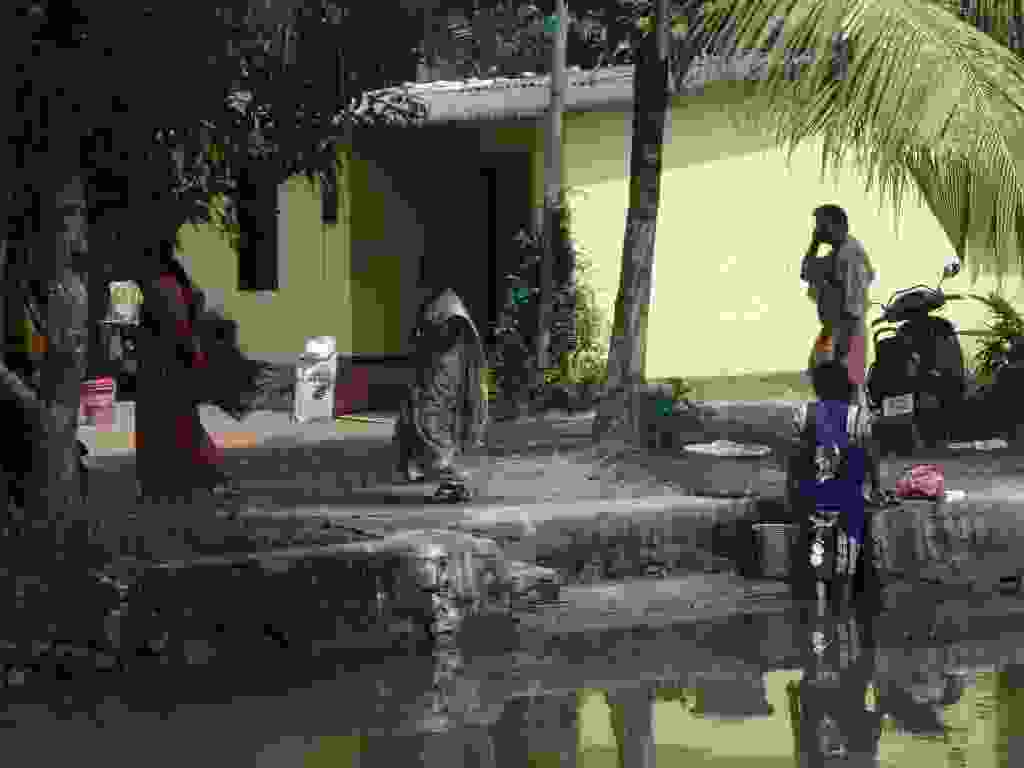
\includegraphics[width=\mywidth]{../wp-content/uploads/2015/11/wpid-oi000235-1024x768.jpg} \end{center}

 

 En descendant du bateau pour se balader on croise un gros lézard 

 

\begin{center} 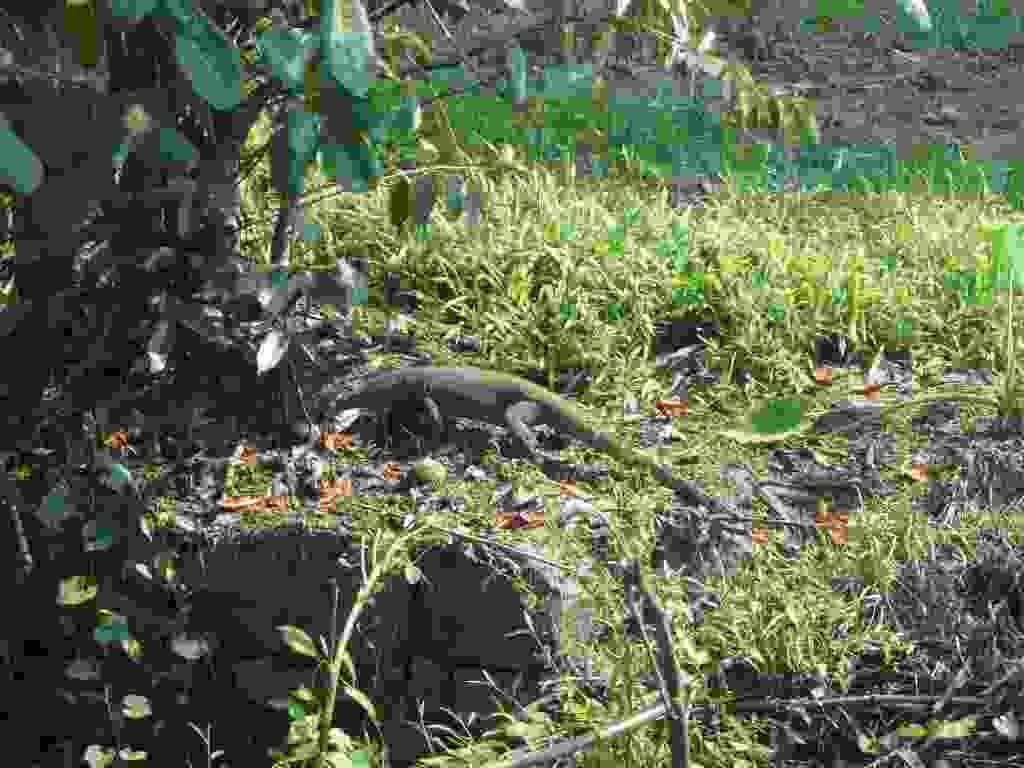
\includegraphics[width=\mywidth]{../wp-content/uploads/2015/11/wpid-oi000244-1024x768.jpg} \end{center}

 

 Je repars en vélo vers l'intérieur des terres, les gens sont amicaux : énormément de saluts à mon passage et souvent des motos viennent rouler à côté de moi pour discuter 

 Beaucoup de grandes maisons souvent bien colorées 

 

\begin{center} 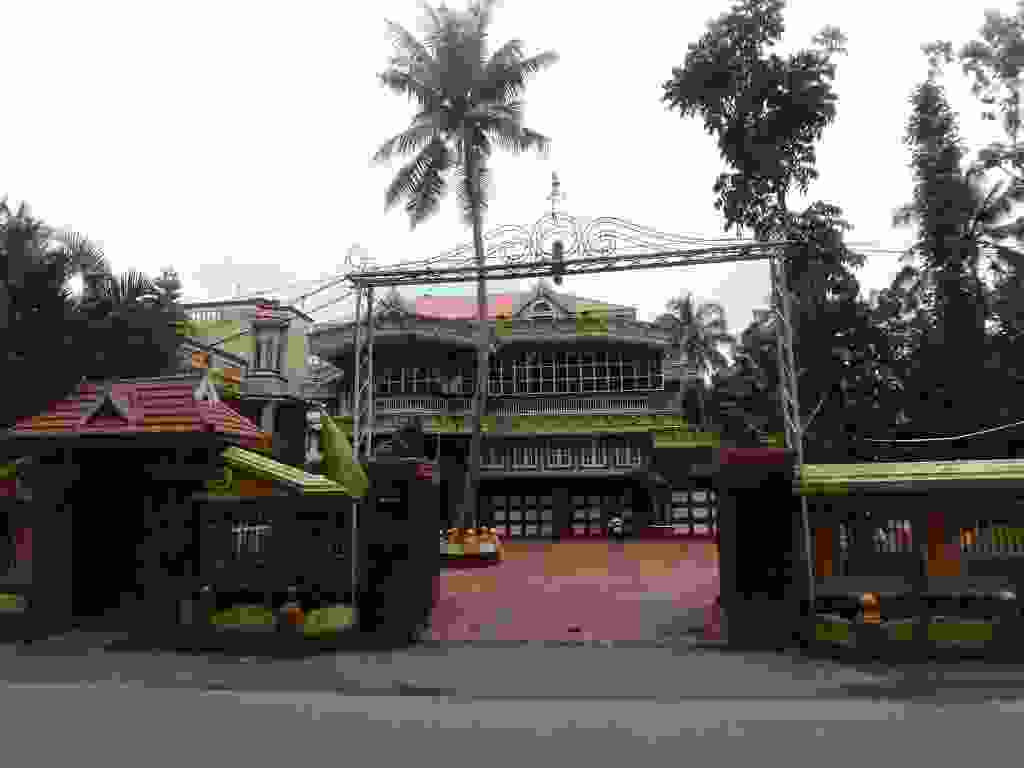
\includegraphics[width=\mywidth]{../wp-content/uploads/2015/11/wpid-oi000260-1024x768.jpg} \end{center}

 

 Encore un pays avec une belle variété de fruits 

 

\begin{center} 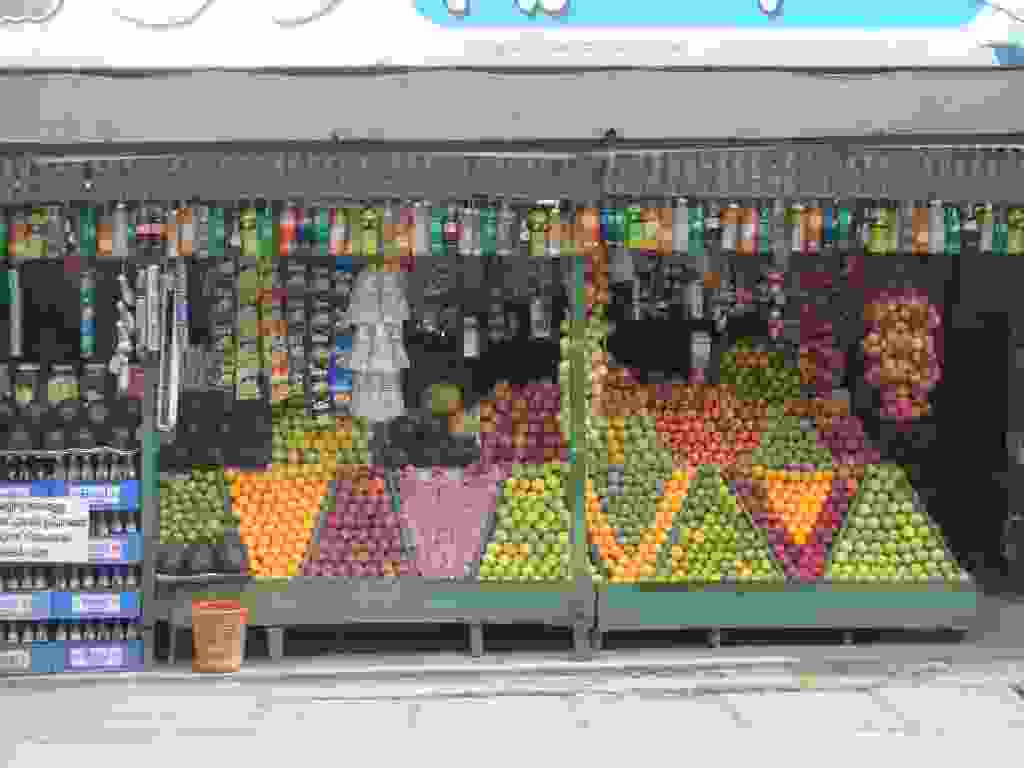
\includegraphics[width=\mywidth]{../wp-content/uploads/2015/11/wpid-oi000262-1024x768.jpg} \end{center}

 

 A côté des cultures d'ananas, le verre de jus frais à 35 centimes ! 

 

\begin{center} 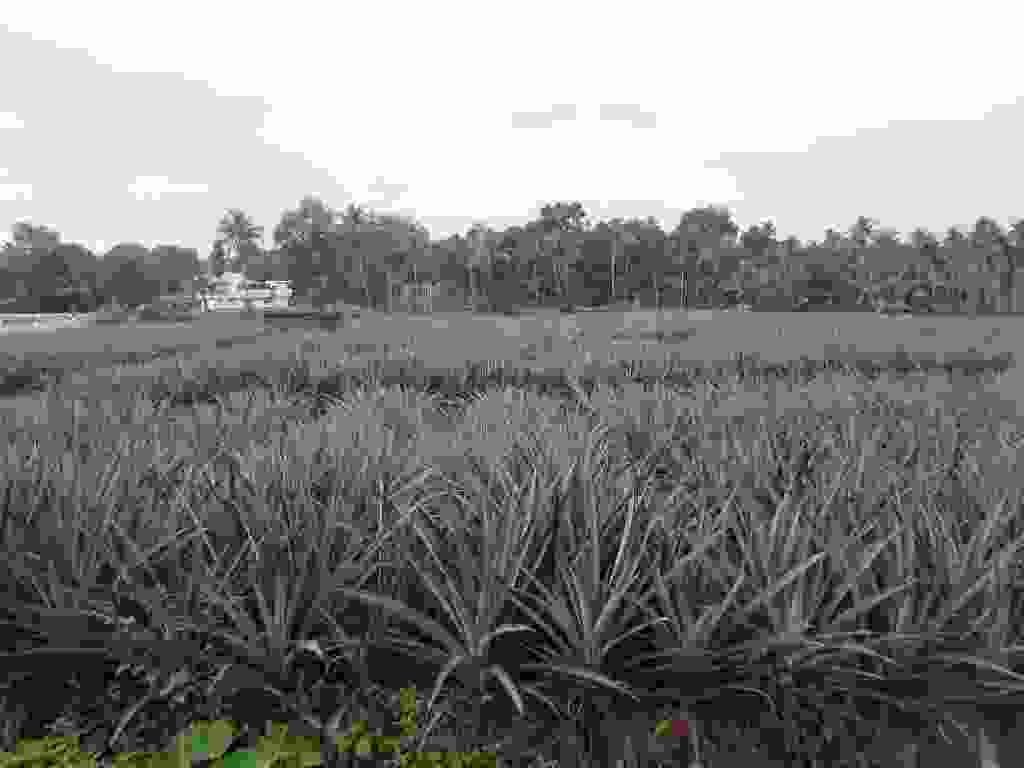
\includegraphics[width=\mywidth]{../wp-content/uploads/2015/11/wpid-oi000264-1024x768.jpg} \end{center}

 

 

\begin{center} 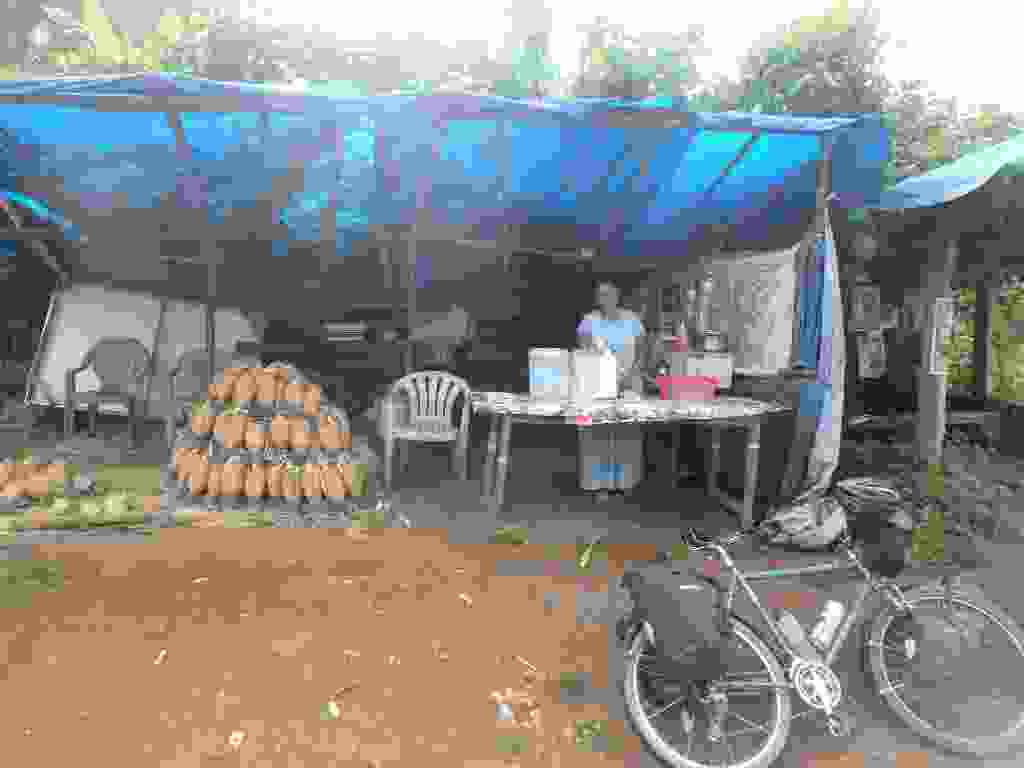
\includegraphics[width=\mywidth]{../wp-content/uploads/2015/11/wpid-oi000263-1024x768.jpg} \end{center}

 

 Je passe devant une répétition de percussions, le prof me fait signe de venir voir 

 

\begin{center} 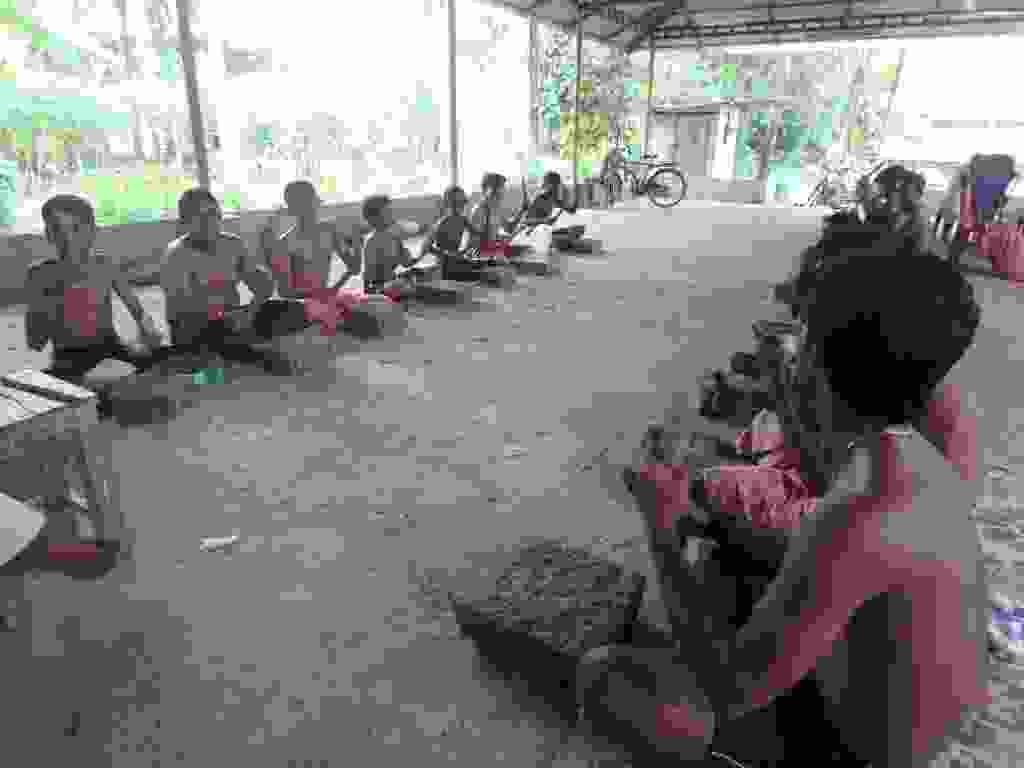
\includegraphics[width=\mywidth]{../wp-content/uploads/2015/11/wpid-oi000266-1024x768.jpg} \end{center}

 

 

\begin{center} 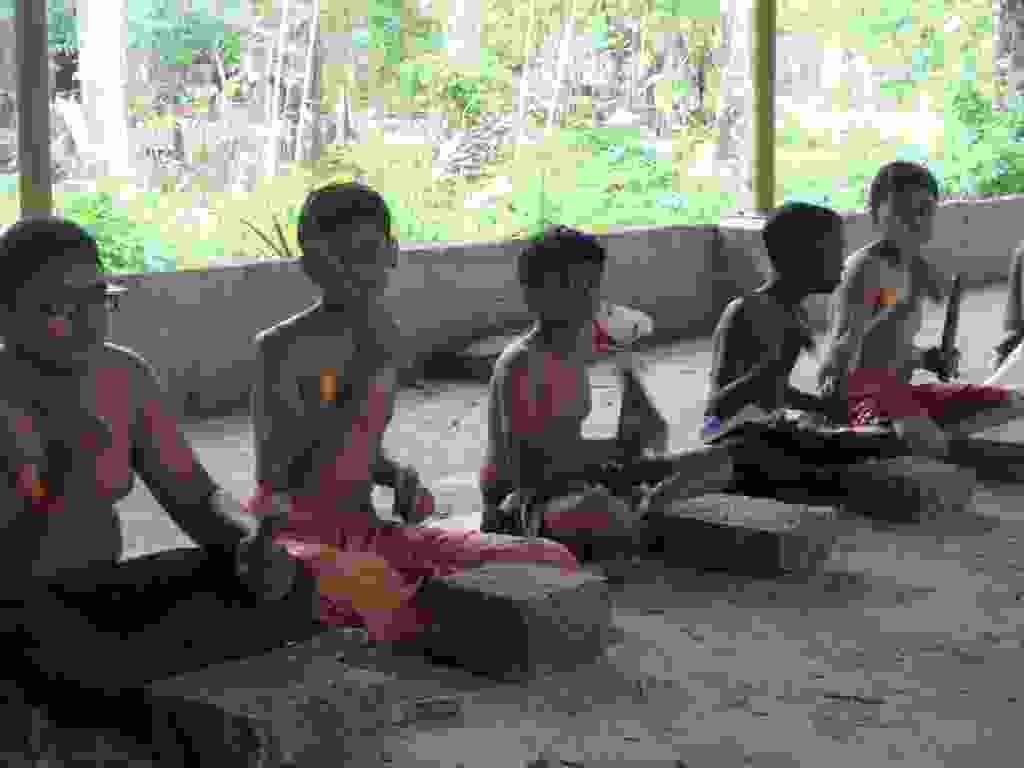
\includegraphics[width=\mywidth]{../wp-content/uploads/2015/11/wpid-oi000267-1024x768.jpg} \end{center}

 

 

\begin{center} 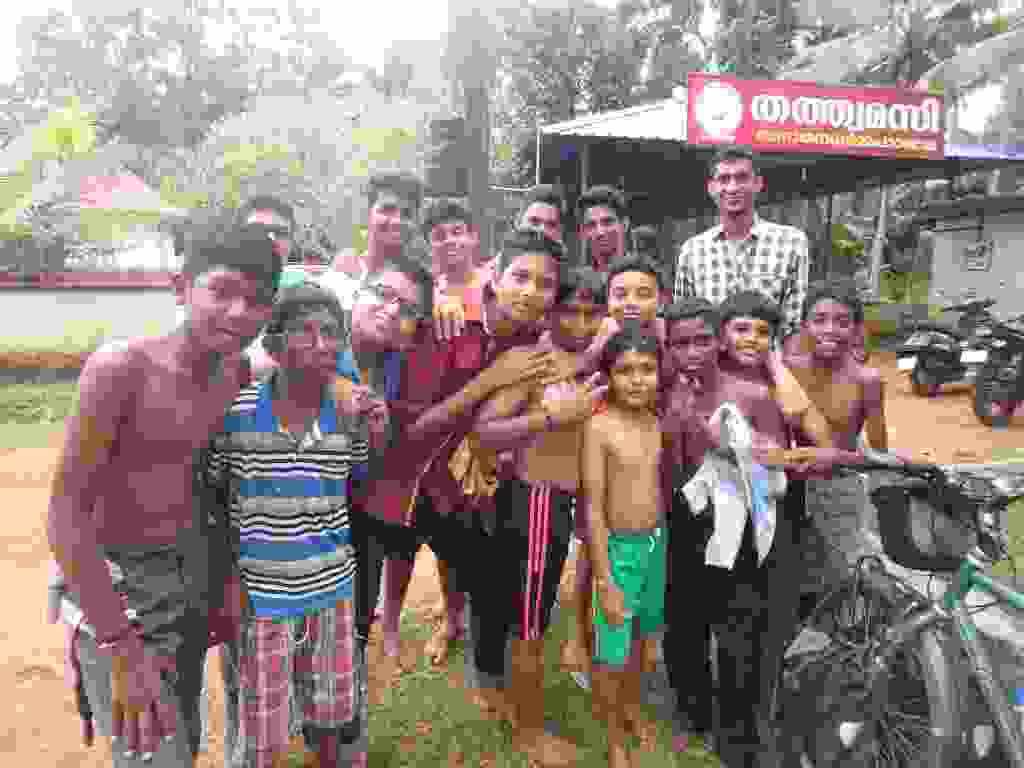
\includegraphics[width=\mywidth]{../wp-content/uploads/2015/11/wpid-oi000269-1024x768.jpg} \end{center}

 

 Arrêt pour visiter un jardin de plantes ayurvédiques 

 

\begin{center} 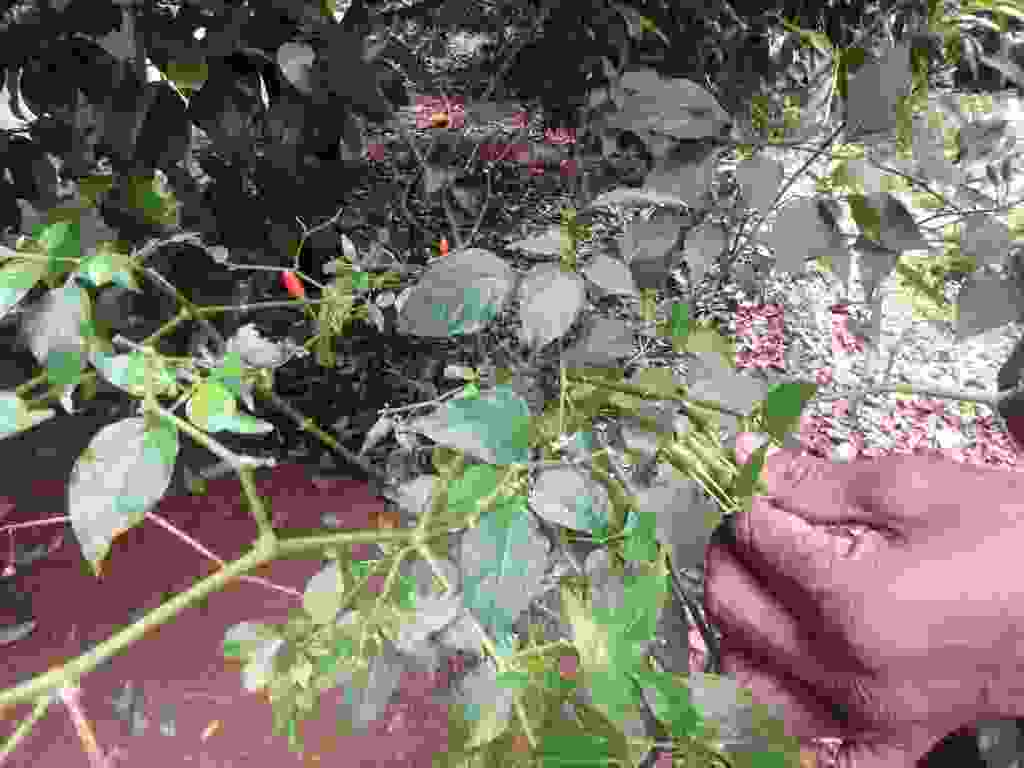
\includegraphics[width=\mywidth]{../wp-content/uploads/2015/11/wpid-oi000280-1024x768.jpg} \end{center}

 

 

\begin{center} 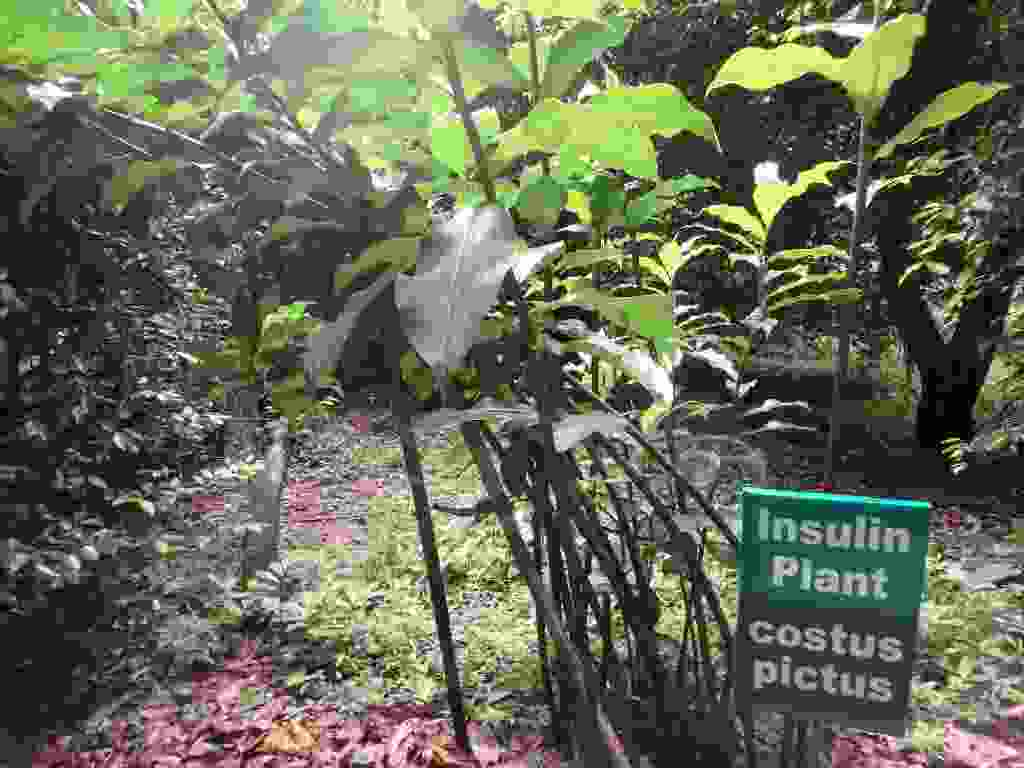
\includegraphics[width=\mywidth]{../wp-content/uploads/2015/11/wpid-oi000289-1024x768.jpg} \end{center}

 

 La route s'élève en s'approchant de Munnar 

 

\begin{center} 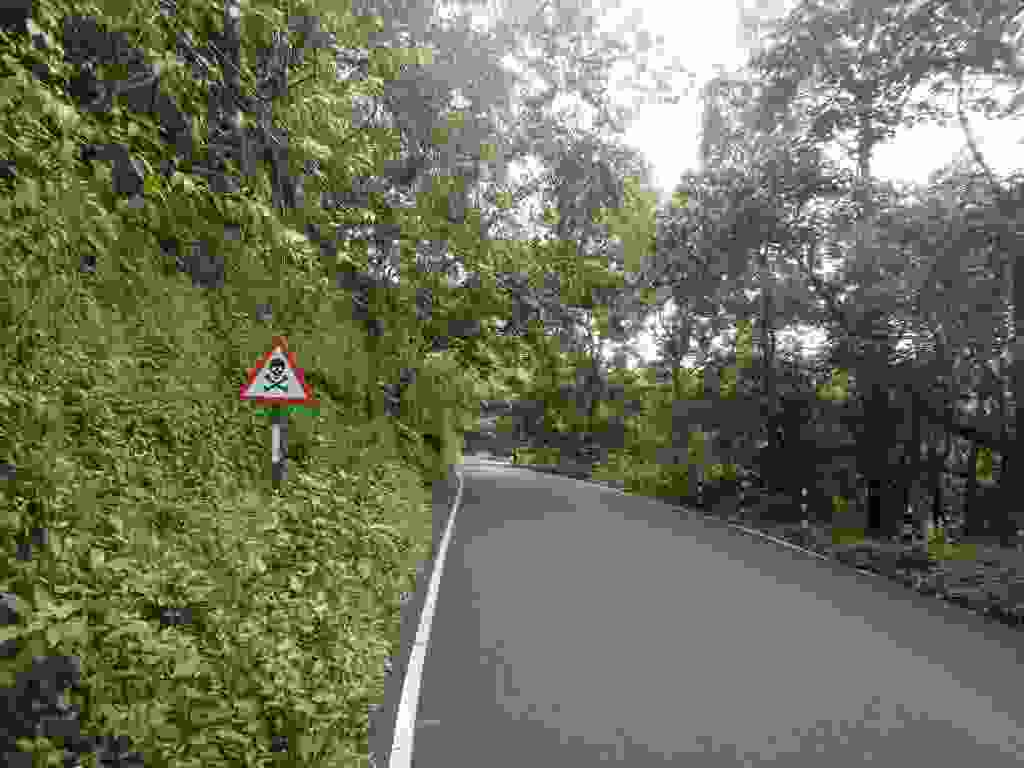
\includegraphics[width=\mywidth]{../wp-content/uploads/2015/11/wpid-oi000272-1024x768.jpg} \end{center}

 

 

\begin{center} 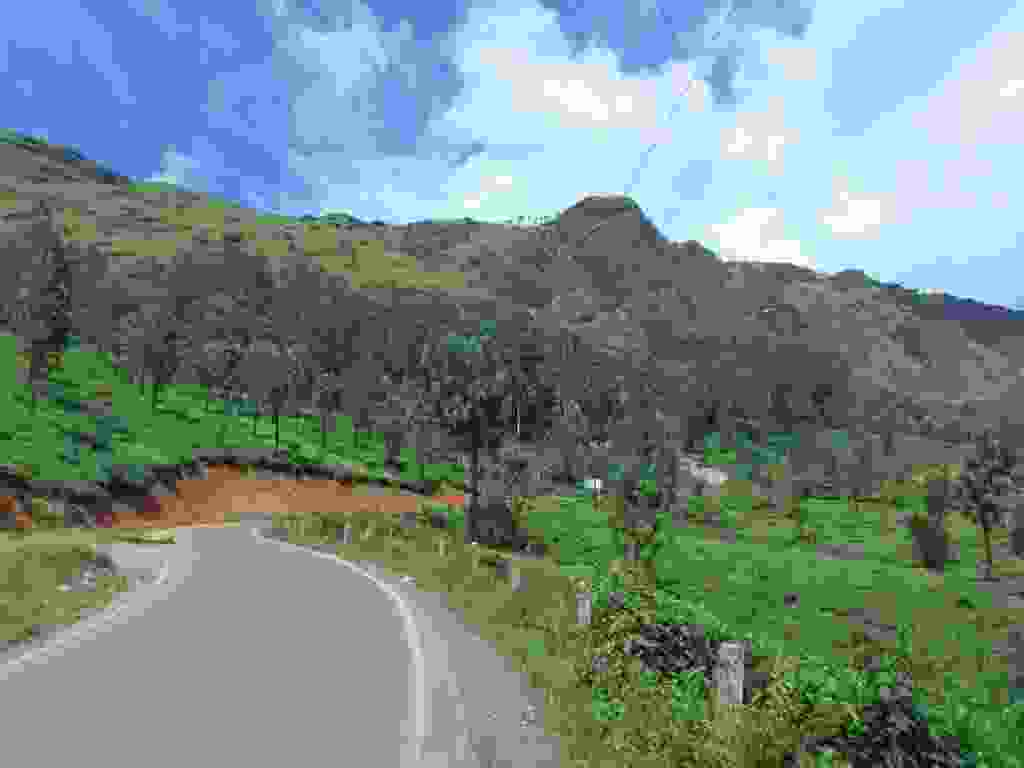
\includegraphics[width=\mywidth]{../wp-content/uploads/2015/11/wpid-oi00021801.jpg-1024x768.jpg} \end{center}

 

 Munnar à environ 1500m d'altitude, un peu de fraîcheur par rapport à la chaleur humide sur la côte 

 

\begin{center} 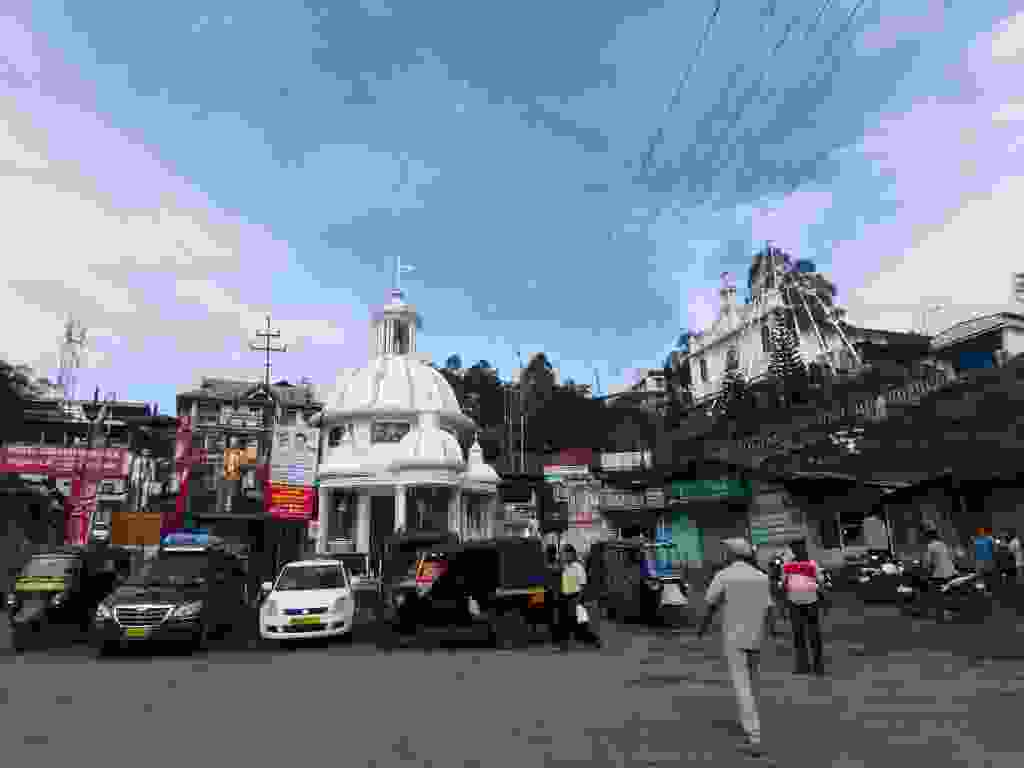
\includegraphics[width=\mywidth]{../wp-content/uploads/2015/11/wpid-oi000293-1024x768.jpg} \end{center}

 

 

\begin{center} 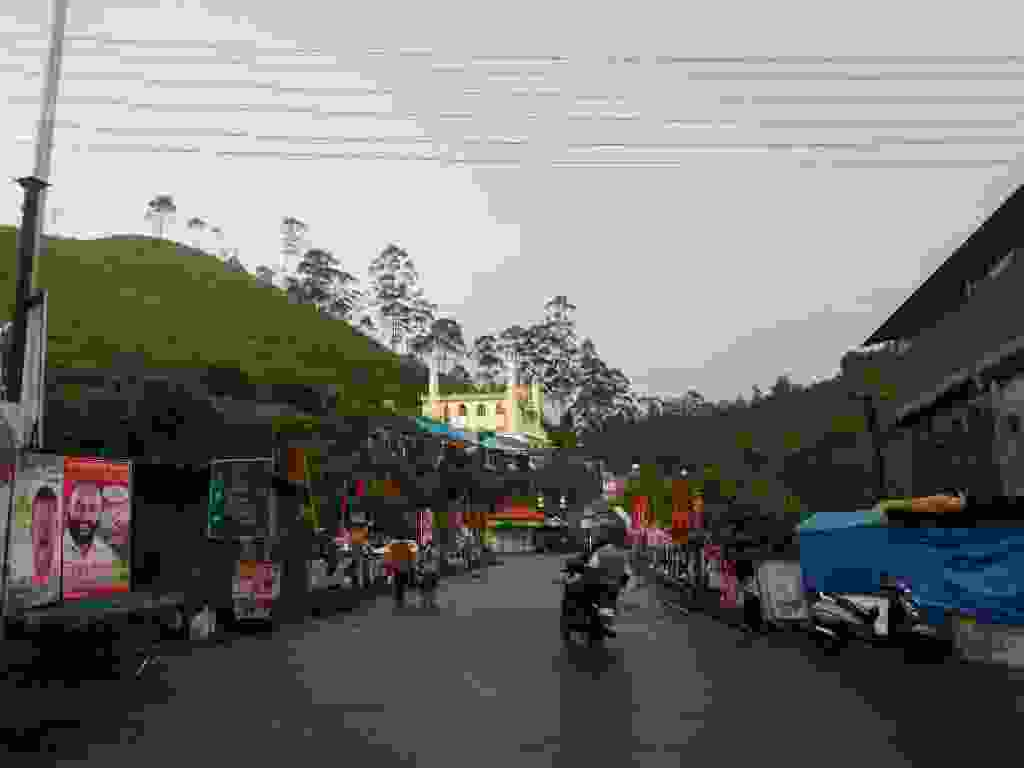
\includegraphics[width=\mywidth]{../wp-content/uploads/2015/11/wpid-oi000308-1024x768.jpg} \end{center}

 

 Les alentours sont couverts de plantations de thé 

 

\begin{center} 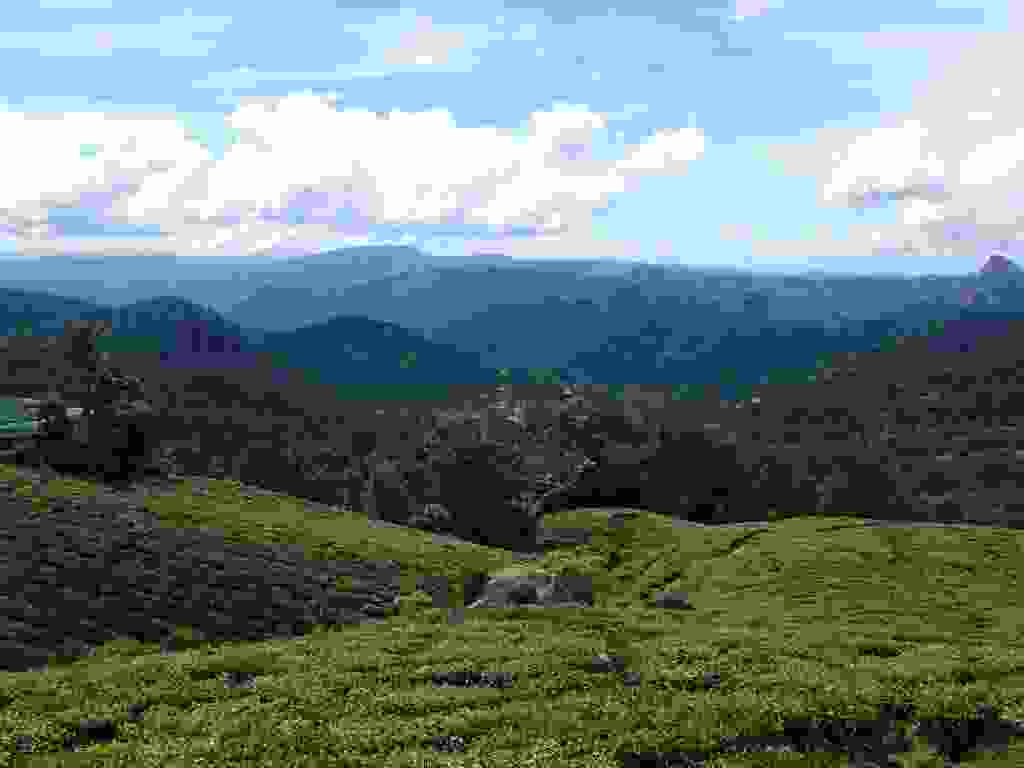
\includegraphics[width=\mywidth]{../wp-content/uploads/2015/11/wpid-oi00023301.jpg-1024x768.jpg} \end{center}

 

 

\begin{center} 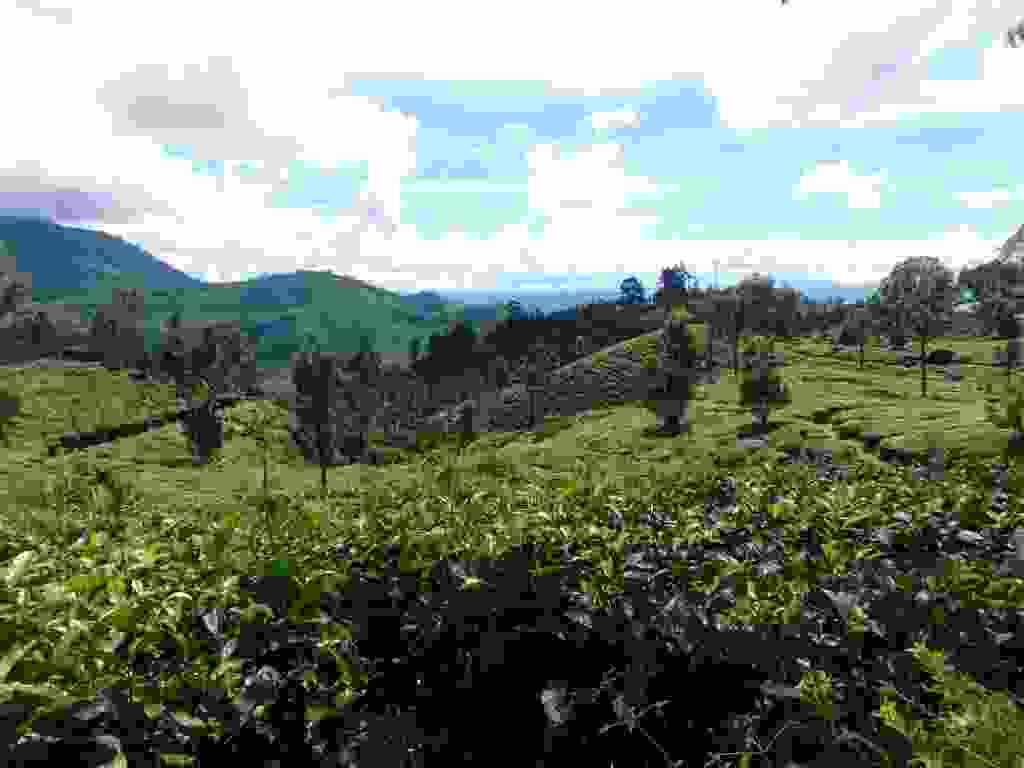
\includegraphics[width=\mywidth]{../wp-content/uploads/2015/11/wpid-oi00021501.jpg-1024x768.jpg} \end{center}

 

 Le musée du thé montre les machines pour fabriquer le thé noir 

 

\begin{center} 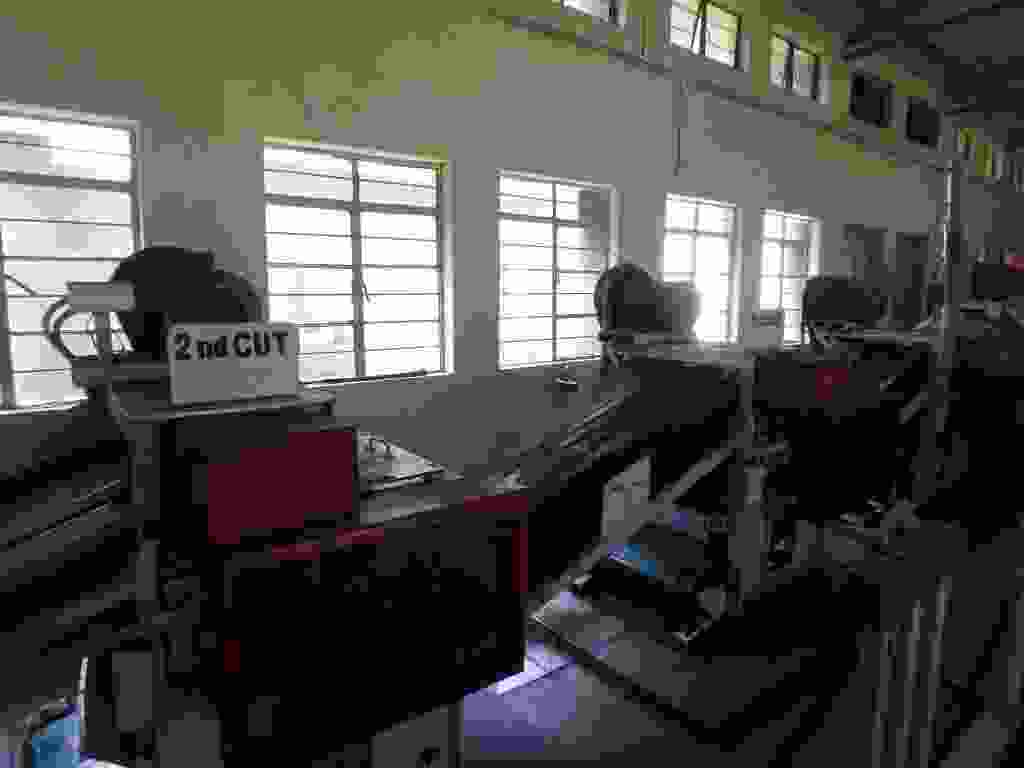
\includegraphics[width=\mywidth]{../wp-content/uploads/2015/11/wpid-oi00018601.jpg-1024x768.jpg} \end{center}

 

 Montée à la Top Station à plus de 2000m, jolie surprise au bord de la route 

 

\begin{center} 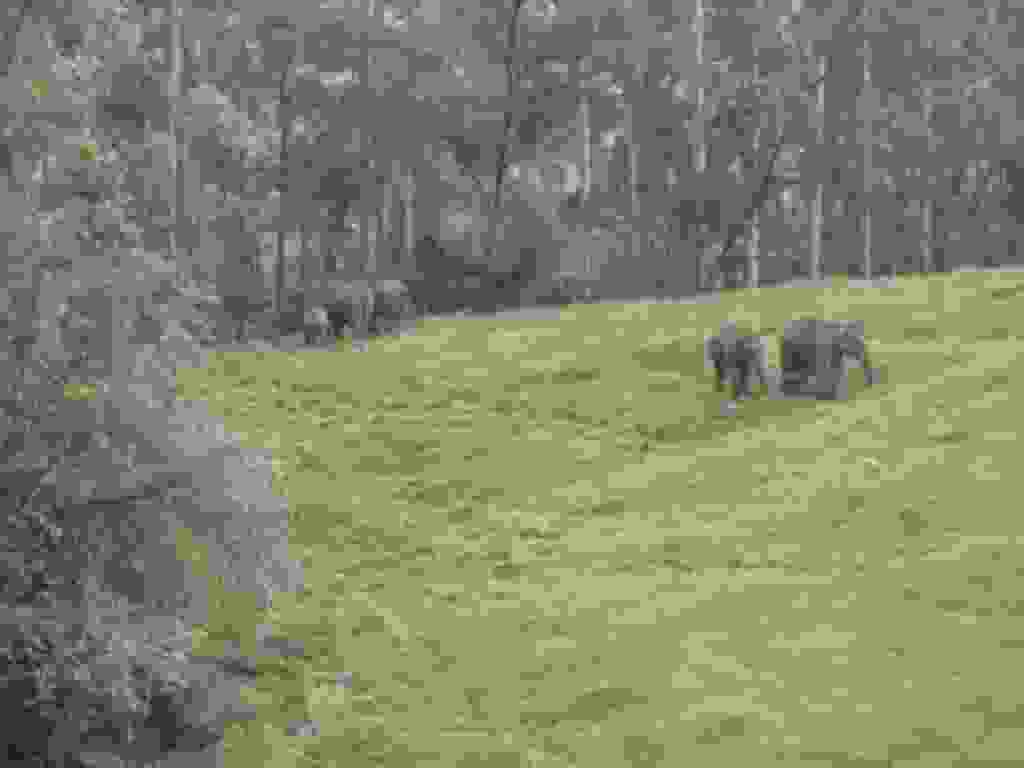
\includegraphics[width=\mywidth]{../wp-content/uploads/2015/11/wpid-oi000299-1024x768.jpg} \end{center}

 

 

\begin{center} 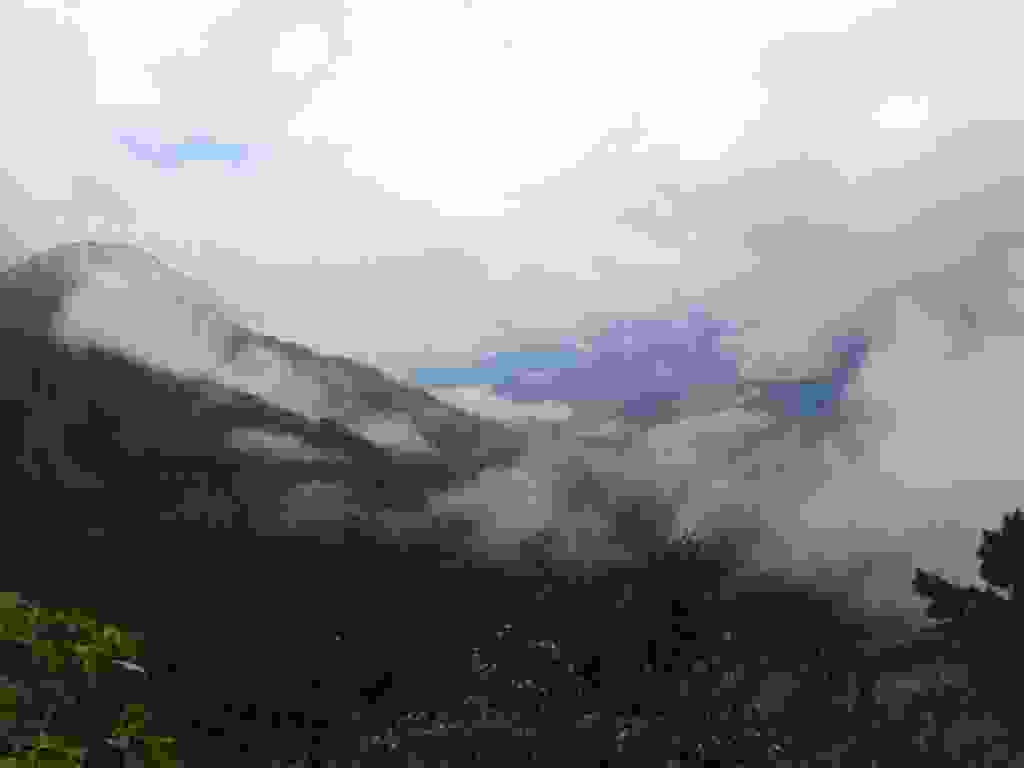
\includegraphics[width=\mywidth]{../wp-content/uploads/2015/11/wpid-oi000302-1024x768.jpg} \end{center}

 

 Côte nourriture plein de choses à tester, un thali pour commencer, à manger avec la main droite bien sûr 

 

\begin{center} 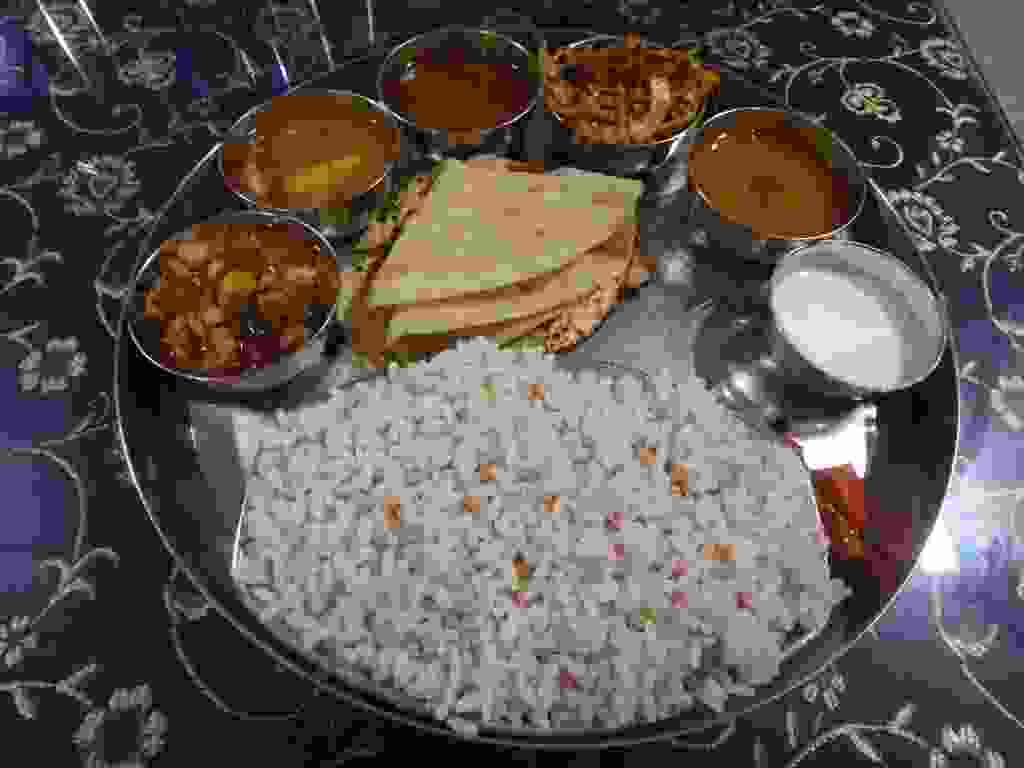
\includegraphics[width=\mywidth]{../wp-content/uploads/2015/11/wpid-oi000270-1024x768.jpg} \end{center}




 
 
